\documentclass[10pt,letterpaper]{article}
\usepackage[utf8]{inputenc}
\usepackage[intlimits]{amsmath}
\usepackage{amsfonts}
\usepackage{amssymb}
\usepackage{ragged2e}
\usepackage[letterpaper, margin=0.5in]{geometry}
\usepackage{graphicx}
\usepackage{cancel}
\usepackage{mathtools}
\usepackage{tabularx}
\usepackage{arydshln}
\usepackage{tensor}
\usepackage{array}
\usepackage{xcolor}
\usepackage[boxed]{algorithm}
\usepackage[noend]{algpseudocode}
\usepackage{listings}
\usepackage{textcomp}
% \usepackage[pdf,tmpdir,singlefile]{graphviz}
\usepackage{mathrsfs}
\usepackage{bbm}
\usepackage{tikz}
\usepackage{tikz-cd}
\usepackage{enumitem}
\usepackage{arydshln}
\usepackage{relsize}
\usepackage{multirow,multicol}
\usepackage{scalerel}
\usepackage{upgreek}
\usepackage{ifthen}

\usetikzlibrary{bayesnet}
\usetikzlibrary{patterns}
\setlist{noitemsep}

%%%%%%%%%%%%%%%%%%%%%%%%%%%%%
% Formatting commands
%%%%%%%%%%%%%%%%%%%%%%%%%%%%%
\newcommand{\n}{\hfill\break}
\newcommand{\nn}{\vspace{0.5\baselineskip}\n}
\newcommand{\up}{\vspace{-\baselineskip}}
\newcommand{\hangblock}[2]{\par\noindent\settowidth{\hangindent}{\textbf{#1: }}\textbf{#1: }\nolinebreak#2}
\newcommand{\lemma}[1]{\hangblock{Lemma}{#1}}
\newcommand{\defn}[1]{\hangblock{Defn}{#1}}
\newcommand{\thm}[1]{\hangblock{Thm}{#1}}
\newcommand{\cor}[1]{\hangblock{Cor}{#1}}
\newcommand{\prop}[1]{\hangblock{Prop}{#1}}
\newcommand{\ex}[1]{\hangblock{Ex}{#1}}
\newcommand{\exer}[1]{\hangblock{Exer}{#1}}
\newcommand{\fact}[1]{\hangblock{Fact}{#1}}
\newcommand{\remark}[1]{\hangblock{Remark}{#1}}
\newcommand{\proven}{\;$\square$\n}
\newcommand{\problem}[1]{\par\noindent{\nolinebreak#1}\n}
\newcommand{\problempart}[2]{\par\noindent\indent{}\settowidth{\hangindent}{\textbf{(#1)} \indent{}}\textbf{(#1) }\nolinebreak#2\n}
\newcommand{\ptxt}[1]{\textrm{\textnormal{#1}}}
\newcommand{\inlineeq}[1]{\centerline{$\displaystyle #1$}}
\newcommand{\pageline}{\up\par\noindent\rule{\textwidth}{0.1pt}}

%%%%%%%%%%%%%%%%%%%%%%%%%%%%%
% Math commands
%%%%%%%%%%%%%%%%%%%%%%%%%%%%%
% Set Theory
\newcommand{\card}[1]{\left|#1\right|}
\newcommand{\set}[1]{\left\{#1\right\}}
\newcommand{\setmid}{\;\middle|\;}
\newcommand{\ps}[1]{\mathcal{P}\left(#1\right)}
\newcommand{\pfinite}[1]{\mathcal{P}^{\ptxt{finite}}\left(#1\right)}
\newcommand{\naturals}{\mathbb{N}}
\newcommand{\N}{\naturals}
\newcommand{\integers}{\mathbb{Z}}
\newcommand{\Z}{\integers}
\newcommand{\rationals}{\mathbb{Q}}
\newcommand{\Q}{\rationals}
\newcommand{\reals}{\mathbb{R}}
\newcommand{\R}{\reals}
\newcommand{\complex}{\mathbb{C}}
\newcommand{\C}{\complex}
\newcommand{\halfPlane}{\mathbb{H}}
\let\HSym\H
\let\H\relax
\newcommand{\H}{\halfPlane}
\newcommand{\comp}{^{\complement}}
\DeclareMathOperator{\Hom}{Hom}
\newcommand{\Ind}{\mathbbm{1}}
\newcommand{\cut}{\setminus}
\DeclareMathOperator{\elem}{elem}

% Differentiable Manifolds
\newcommand{\RP}{\mathbb{RP}}
\newcommand{\CP}{\mathbb{RP}}
\newcommand{\osubset}{\overset{\mathclap{\scalebox{0.5}{\ptxt{open}}}}{\subset}}
\newcommand{\osubseteq}{\overset{\mathclap{\scalebox{0.5}{\ptxt{open}}}}{\subseteq}}
\newcommand{\osupset}{\overset{\mathclap{\scalebox{0.5}{\ptxt{open}}}}{\supset}}
\newcommand{\osupseteq}{\overset{\mathclap{\scalebox{0.5}{\ptxt{open}}}}{\supseteq}}
\newcommand{\pdat}[3]{\left.\pd{#1}{#2}\right|_{#3}}
\DeclareMathOperator{\so}{so}
\DeclareMathOperator{\codim}{codim}
\DeclareMathOperator{\Diff}{Diff}
\let\dSym\d
\let\d\relax
\newcommand{\d}{\partial}
\DeclareMathOperator{\gl}{gl}
\DeclareMathOperator{\Ad}{Ad}
\newcommand{\comm}[1]{\left[#1\right]}
\DeclareMathOperator{\Fix}{Fix}

% Graph Theory
\let\deg\relax
\DeclareMathOperator{\deg}{deg}
\newcommand{\degp}{\ptxt{deg}^{+}}
\newcommand{\degn}{\ptxt{deg}^{-}}
\newcommand{\precdot}{\mathrel{\ooalign{$\prec$\cr\hidewidth\hbox{$\cdot\mkern0.5mu$}\cr}}}
\newcommand{\succdot}{\mathrel{\ooalign{$\cdot\mkern0.5mu$\cr\hidewidth\hbox{$\succ$}\cr\phantom{$\succ$}}}}
\DeclareMathOperator{\cl}{cl}
\DeclareMathOperator{\affdim}{affdim}

% Probability
\newcommand{\parSymbol}{\P}
\newcommand{\Prob}{\mathbb{P}}
\renewcommand{\P}{\Prob}
\newcommand{\Avg}{\mathbb{E}}
\newcommand{\E}{\Avg}
\DeclareMathOperator{\Var}{Var}
\DeclareMathOperator{\Cov}{Cov}
\DeclareMathOperator{\cov}{cov}
\DeclareMathOperator{\Corr}{Corr}
\DeclareMathOperator{\Unif}{Unif}
\DeclareMathOperator{\Binom}{Binom}
\newcommand{\CI}{\mathrel{\text{\scalebox{1.07}{$\perp\mkern-10mu\perp$}}}}
\DeclareMathOperator{\Ber}{Ber}
\DeclareMathOperator{\Bin}{Bin}
\DeclareMathOperator{\Geom}{Geom}
\DeclareMathOperator{\Poisson}{Poisson}
\DeclareMathOperator{\Exp}{Exp}
\DeclareMathOperator{\Beta}{Beta}
\DeclareMathOperator{\Normal}{N}
\DeclareMathOperator{\DistGamma}{Gamma}

% Standard Math
\newcommand{\inv}{^{-1}}
\newcommand{\abs}[1]{\left|#1\right|}
\newcommand{\ceil}[1]{\left\lceil{}#1\right\rceil{}}
\newcommand{\floor}[1]{\left\lfloor{}#1\right\rfloor{}}
\newcommand{\conj}[1]{\overline{#1}}
\newcommand{\of}{\circ}
\newcommand{\tri}{\triangle}
\newcommand{\inj}{\hookrightarrow}
\newcommand{\surj}{\twoheadrightarrow}
\newcommand{\ndiv}{\nmid}
\renewcommand{\epsilon}{\varepsilon}
\newcommand{\divides}{\mid}
\newcommand{\ndivides}{\nmid}
\DeclareMathOperator{\lcm}{lcm}
\DeclareMathOperator{\sgn}{sgn}
\newcommand{\map}[4]{\!\!\!\begin{array}[t]{rcl}#1 & \!\!\!\!\to & \!\!\!\!#2\\ {}#3 & \!\!\!\!\mapsto & \!\!\!\!#4\end{array}}
\newcommand{\bigsum}[2]{\smashoperator[lr]{\sum_{\scalebox{#1}{$#2$}}}}
\DeclareMathOperator{\gcf}{gcf}
\newcommand{\restr}[1]{\left.#1\right|}

% Linear Algebra
\newcommand{\Id}{\textrm{\textnormal{Id}}}
\newcommand{\im}{\textrm{\textnormal{im}}}
\newcommand{\norm}[1]{\abs{\abs{#1}}}
\newcommand{\tpose}{^{T}\!}
\newcommand{\iprod}[1]{\left<#1\right>}
\newcommand{\giprod}{\iprod{\;\,,\;}}
\DeclareMathOperator{\tr}{tr}
\DeclareMathOperator{\trace}{tr}
\newcommand{\chgBasMat}[3]{\!\!\tensor*[_{#1}]{\left[#2\right]}{_{#3}}}
\newcommand{\vecBas}[2]{\tensor*[]{\left[#1\right]}{_{#2}}}
\DeclareMathOperator{\GL}{GL}
\DeclareMathOperator{\Mat}{Mat}
\DeclareMathOperator{\vspan}{span}
\DeclareMathOperator{\rank}{rank}
\newcommand{\V}[1]{\vec{#1}}
\DeclareMathOperator{\proj}{proj}
\DeclareMathOperator{\compProj}{comp}
\DeclareMathOperator{\row}{row}
\newcommand{\smallPMatrix}[1]{\paren{\begin{smallmatrix}#1\end{smallmatrix}}}
\newcommand{\smallBMatrix}[1]{\brack{\begin{smallmatrix}#1\end{smallmatrix}}}
\newcommand{\pmat}[1]{\begin{pmatrix}#1\end{pmatrix}}
\newcommand{\bmat}[1]{\begin{bmatrix}#1\end{bmatrix}}
\newcommand{\dual}{^{*}}
\newcommand{\pinv}{^{\dagger}}
\newcommand{\horizontalMatrixLine}{\ptxt{\rotatebox[origin=c]{-90}{$|$}}}
\DeclareMathOperator{\range}{range}
\DeclareMathOperator{\Symm}{Symm}
\DeclareMathOperator{\SU}{SU}
\DeclareMathOperator{\U}{U}

% Multilinear Algebra
\let\Lsym\L
\let\L\relax
\DeclareMathOperator{\L}{\mathscr{L}}
\DeclareMathOperator{\A}{\mathcal{A}}
\DeclareMathOperator{\Alt}{Alt}
\DeclareMathOperator{\Sym}{Sym}
\newcommand{\ot}{\otimes}
\newcommand{\ox}{\otimes}
\DeclareMathOperator{\asc}{asc}
\DeclareMathOperator{\asSet}{set}
\DeclareMathOperator{\sort}{sort}
\DeclareMathOperator{\ringA}{\mathring{A}}
\DeclareMathOperator{\Sh}{Sh}
\DeclareMathOperator{\Bil}{Bil}

% Topology
\newcommand{\closure}[1]{\overline{#1}}
\newcommand{\uball}{\mathcal{U}}
\DeclareMathOperator{\Int}{Int}
\DeclareMathOperator{\Ext}{Ext}
\DeclareMathOperator{\Bd}{Bd}
\DeclareMathOperator{\rInt}{rInt}
\DeclareMathOperator{\ch}{ch}
\DeclareMathOperator{\ah}{ah}
\newcommand{\LargerTau}{\mathlarger{\mathlarger{\mathlarger{\mathlarger{\tau}}}}}
\newcommand{\Tau}{\mathcal{T}}

% Analysis
\DeclareMathOperator{\Graph}{Graph}
\DeclareMathOperator{\epi}{epi}
\DeclareMathOperator{\hypo}{hypo}
\DeclareMathOperator{\supp}{supp}
\newcommand{\lint}[2]{\underset{#1}{\overset{#2}{{\color{black}\underline{{\color{white}\overline{{\color{black}\int}}\color{black}}}}}}}
\newcommand{\uint}[2]{\underset{#1}{\overset{#2}{{\color{white}\underline{{\color{black}\overline{{\color{black}\int}}\color{black}}}}}}}
\newcommand{\alignint}[2]{\underset{#1}{\overset{#2}{{\color{white}\underline{{\color{white}\overline{{\color{black}\int}}\color{black}}}}}}}
\newcommand{\extint}{\ptxt{ext}\int}
\newcommand{\extalignint}[2]{\ptxt{ext}\alignint{#1}{#2}}
\newcommand{\conv}{\ast}
\newcommand{\pd}[2]{\frac{\partial{}#1}{\partial{}#2}}
\newcommand{\del}{\nabla}
\DeclareMathOperator{\grad}{grad}
\DeclareMathOperator{\curl}{curl}
\let\div\relax
\DeclareMathOperator{\div}{div}
\DeclareMathOperator{\vol}{vol}

% Complex Analysis
\let\Re\relax
\DeclareMathOperator{\Re}{Re}
\let\Im\relax
\DeclareMathOperator{\Im}{Im}
\DeclareMathOperator{\Res}{Res}

% Abstract Algebra
\DeclareMathOperator{\ord}{ord}
\newcommand{\generated}[1]{\left<#1\right>}
\newcommand{\cycle}[1]{\smallPMatrix{#1}}
\newcommand{\id}{\ptxt{id}}
\newcommand{\iso}{\cong}
\DeclareMathOperator{\Aut}{Aut}
\DeclareMathOperator{\SL}{SL}
\DeclareMathOperator{\op}{op}
\newcommand{\isom}[4]{\!\!\!\begin{array}[t]{rcl}#1 & \!\!\!\!\overset{\sim}{\to} & \!\!\!\!#2\\ #3 & \!\!\!\!\mapsto & \!\!\!\!#4\end{array}}
\newcommand{\F}{\mathbb{F}}
\newcommand{\acts}{\;\reflectbox{\rotatebox[origin=c]{-90}{$\circlearrowright$}}\;}
\newcommand{\disjunion}{\mathrel{\text{\scalebox{1.07}{$\perp\mkern-10mu\perp$}}}}
\DeclareMathOperator{\SO}{SO}
\DeclareMathOperator{\stab}{stab}
\DeclareMathOperator{\nullity}{nullity}
\DeclareMathOperator{\Perm}{Perm}
\DeclareMathOperator{\nsubgp}{\vartriangleleft}
\DeclareMathOperator{\notnsubgp}{\ntriangleleft}
\newcommand{\presentation}[2]{\left<#1\;\middle|\;#2\right>}
\DeclareMathOperator{\Char}{char}
\DeclareMathOperator{\fchar}{char}
\DeclareMathOperator{\triv}{triv}
\DeclareMathOperator{\reg}{reg}
\DeclareMathOperator{\std}{std}
\DeclareMathOperator{\Func}{Func}
\DeclareMathOperator{\End}{End}

% Convex Optimization
\let\sectionSymbol\S
\let\S\relax
\newcommand{\S}{\mathbb{S}}
\DeclareMathOperator{\dist}{dist}
\DeclareMathOperator{\dom}{dom}
\DeclareMathOperator{\diag}{diag}
\DeclareMathOperator{\ones}{\mathbbm{1}}
\newcommand{\minimizeOver}[3]{\begin{array}{rl}\underset{#1}{\ptxt{minimize}} & #2\\ \ptxt{subject to} & #3\end{array}}
\newcommand{\maximizeOver}[3]{\begin{array}{rl}\underset{#1}{\ptxt{maximize}} & #2\\ \ptxt{subject to} & #3\end{array}}
\newcommand{\minimizationProblem}[2]{\minimizeOver{}{#1}{#2}}
\newcommand{\maximizationProblem}[2]{\maximizeOver{}{#1}{#2}}
\newcommand{\minimizeOverUnconstrained}[2]{\begin{array}{rl}\underset{#1}{\ptxt{minimize}} & #2\end{array}}
\newcommand{\maximizeOverUnconstrained}[2]{\begin{array}{rl}\underset{#1}{\ptxt{maximize}} & #2\end{array}}
\newcommand{\minimizationUnconstrained}[1]{\minimizeOverUnconstrained{}{#1}}
\newcommand{\maximizationUnconstrained}[1]{\maximizeOverUnconstrained{}{#1}}
\DeclareMathOperator{\argmin}{argmin}
\DeclareMathOperator{\argmax}{argmax}

% Proofs
\newcommand{\st}{s.t.}
\newcommand{\unique}{!}
\newcommand{\iffdef}{\overset{\ptxt{def}}{\Leftrightarrow}}
\newcommand{\eqVertical}{\rotatebox[origin=c]{90}{=}}
\newcommand{\mapsfrom}{\mathrel{\reflectbox{\ensuremath{\mapsto}}}}
\newcommand{\mapsdown}{\rotatebox[origin=c]{-90}{$\mapsto$}\mkern2mu}
\newcommand{\mapsup}{\rotatebox[origin=c]{90}{$\mapsto$}\mkern2mu}
\newcommand{\from}{\!\mathrel{\reflectbox{\ensuremath{\to}}}}
\newcommand{\labeledeq}[1]{\overset{\mathclap{\ptxt{#1}}}{=}}
\newcommand{\eqdef}{\labeledeq{def}}

% Brackets
\newcommand{\paren}[1]{\left(#1\right)}
\renewcommand{\brack}[1]{\left[#1\right]}
\renewcommand{\brace}[1]{\left\{#1\right\}}
\newcommand{\ang}[1]{\left<#1\right>}

% Algorithms
\algrenewcommand{\algorithmiccomment}[1]{\hskip 1em \texttt{// #1}}
\algrenewcommand\algorithmicrequire{\textbf{Input:}}
\algrenewcommand\algorithmicensure{\textbf{Output:}}
\newcommand{\algP}{\ptxt{\textbf{P}}}
\newcommand{\algNP}{\ptxt{\textbf{NP}}}
\newcommand{\algNPC}{\ptxt{\textbf{NP-Complete}}}
\newcommand{\algNPH}{\ptxt{\textbf{NP-Hard}}}
\newcommand{\algEXP}{\ptxt{\textbf{EXP}}}
\DeclareMathOperator{\fl}{fl}

%%%%%%%%%%%%%%%%%%%%%%%%%%%%%
% Other commands and shorthand
%%%%%%%%%%%%%%%%%%%%%%%%%%%%%
\newcommand{\flag}[1]{\textbf{\textcolor{red}{#1}}}
\let\uSym\u
\let\u\relax
\newcommand{\u}[1]{\underline{#1}}
\let\bSym\b
\let\b\relax
\newcommand{\b}[1]{\textbf{#1}}
\let\iSym\i
\let\i\relax
\newcommand{\i}[1]{\textit{#1}}
\let\scSym\sc
\let\sc\relax
\newcommand{\sc}[1]{\textsc{#1}}
\newcommand{\mf}[1]{\mathfrak{#1}}
\newcommand{\mc}[1]{\mathcal{#1}}

%%%%%%%%%%%%%%%%%%%%%%%%%%%%%%%%%%%%%%%
% Make l's curvy in math environments %
%%%%%%%%%%%%%%%%%%%%%%%%%%%%%%%%%%%%%%%
\mathcode`l="8000
\begingroup
\makeatletter
\lccode`\~=`\l
\DeclareMathSymbol{\lsb@l}{\mathalpha}{letters}{`l}
\lowercase{\gdef~{\ifnum\the\mathgroup=\m@ne \ell \else \lsb@l \fi}}%
\endgroup

%%%%%%%%%%%%%%%%%%%%%%%%%
% Fix \vdots and \ddots %
%%%%%%%%%%%%%%%%%%%%%%%%%
\usepackage{letltxmacro}
\LetLtxMacro\orgvdots\vdots
\LetLtxMacro\orgddots\ddots

\makeatletter
\DeclareRobustCommand\vdots{%
	\mathpalette\@vdots{}%
}
\newcommand*{\@vdots}[2]{%
	% #1: math style
	% #2: unused
	\sbox0{$#1\cdotp\cdotp\cdotp\m@th$}%
	\sbox2{$#1.\m@th$}%
	\vbox{%
		\dimen@=\wd0 %
		\advance\dimen@ -3\ht2 %
		\kern.5\dimen@
		% remove side bearings
		\dimen@=\wd2 %
		\advance\dimen@ -\ht2 %
		\dimen2=\wd0 %
		\advance\dimen2 -\dimen@
		\vbox to \dimen2{%
			\offinterlineskip
			\copy2 \vfill\copy2 \vfill\copy2 %
		}%
	}%
}
\DeclareRobustCommand\ddots{%
	\mathinner{%
		\mathpalette\@ddots{}%
		\mkern\thinmuskip
	}%
}
\newcommand*{\@ddots}[2]{%
	% #1: math style
	% #2: unused
	\sbox0{$#1\cdotp\cdotp\cdotp\m@th$}%
	\sbox2{$#1.\m@th$}%
	\vbox{%
		\dimen@=\wd0 %
		\advance\dimen@ -3\ht2 %
		\kern.5\dimen@
		% remove side bearings
		\dimen@=\wd2 %
		\advance\dimen@ -\ht2 %
		\dimen2=\wd0 %
		\advance\dimen2 -\dimen@
		\vbox to \dimen2{%
			\offinterlineskip
			\hbox{$#1\mathpunct{.}\m@th$}%
			\vfill
			\hbox{$#1\mathpunct{\kern\wd2}\mathpunct{.}\m@th$}%
			\vfill
			\hbox{$#1\mathpunct{\kern\wd2}\mathpunct{\kern\wd2}\mathpunct{.}\m@th$}%
		}%
	}%
}
\makeatother

\newcommand{\B}{
	
\begin{tikzpicture}
	\filldraw [fill=red, draw=black] (0, 0) rectangle (0.37, 0.45);
	\draw [line width=0.5mm, white ] (0.1,0.08) -- (0.1,0.38);
	\draw[line width=0.5mm, white ] (0.1, 0.35) .. controls (0.2, 0.35) and (0.4, 0.2625) .. (0.1, 0.225);
	\draw[line width=0.5mm, white ] (0.1, 0.225) .. controls (0.2, 0.225) and (0.4, 0.1625) .. (0.1, 0.1);
	\end{tikzpicture}
}

% Allow custom symbols as arrows in tikz-cd
\tikzset{
  symbol/.style={
    draw=none,
    every to/.append style={
      edge node={node [sloped, allow upside down, auto=false]{$#1$}}}
  }
}
% Example: \arrow[r,symbol=\cong]
% https://tex.stackexchange.com/questions/394154/how-to-include-inclusion-subgroup-relationship-in-tikz-cd-diagram

\author{Professor Alejandro Uribe-Ahumada\\ \small\i{Transcribed by Thomas Cohn}}
\title{Math 635 Lecture 16}
\date{2/26/21} % Can also use \today

\begin{document}
\maketitle
\setlength\RaggedRightParindent{\parindent}
\RaggedRight

\par\noindent
Notation: For $M$, a Riemannian manifold, the map $t\mapsto{}G(t,p,v)$ for $p\in{}M$, $v\in{}T_{p}M$, denotes the geodesic with initial conditions $(p,v)$. We saw that, $\forall{}c\in\R$, if defined, $G(t,p,cv)=G(ct,p,v)$.\n

\par\noindent
We also had the theorem that $\forall{}p\in{}M$, $\exists\varepsilon>0$ \st{} $\forall{}v\in{}B_{0}(\varepsilon)\subseteq{}T_{p}M$ (recall that $B_{0}(\varepsilon)=\set{v\in{}T_{p}M:\norm{v}<\varepsilon}$), $G(t,p,v)$ is defined for $t\in[0,1]$. Based on that fact, we define $\exp_{p}(v)=G(1,p,v)$.\n

\lemma{
	$d(\exp_{p})_{v=0}=\Id_{T_{p}M}$.\n
}

\cor{
	$\forall{}p\in{}M$, $\exists\varepsilon>0$ \st{} $\exp_{p}:B_{0}(\varepsilon)\to{}M$ is a diffeomorphism onto its (open) image $U=\exp_{p}(B_{0}(\varepsilon))$.\n
}

\defn{
	Such a neighborhood $U$ of $p$ is called a \u{normal neighborhood} of $p$.\n
}

\par\noindent
Warning: ``Normal neighborhood'' sometimes means any neighborhood that is the diffeomorphic image by $\exp_{p}$ of a neighborhood of $0\in{}T_{p}M$.\n

\defn{
	\u{Normal coordinates} centered at $p\in{}M$ are any coordinates $(x^{1},\ldots,x^{n})$ of the form
	\[
		\begin{tikzcd}[ampersand replacement=\&]
			% U \arrow[rr, bend right=25, ""{coordinate, name=Z}] \arrow[rr, swap, to path={-- (\tikztostart.south) |- (Z) -|(\tikztotarget.south)}] \arrow[r,"(\exp_{p})\inv"] \&[10pt] T_{p}M \arrow[r,"\sim"] \&[10pt] \R^{n}\\
			% "(x^{1}{,}\ldots{,}x^{n})"
			U \arrow[r,"(\exp_{p})\inv"] \&[15pt] T_{p}M \arrow[r,"\sim"] \arrow[start anchor={[xshift=-10pt]west}, end anchor={south}, bend right=90, ""{coordinate, name=Z1}, phantom] \arrow[start anchor={[xshift=10pt]east}, end anchor={south}, bend left=90, ""{coordinate, name=Z2}, phantom] \&[15pt] \R^{n} \arrow[ll, to path={
				-- (\tikztostart.south)
				|- (Z2)
				-- (Z1)\tikztonodes
				-| (\tikztotarget.south)
				-- (\tikztotarget.south)
			}, leftarrow, "{(x^{1},\ldots,x^{n})}"]
		\end{tikzcd}
	\]
	where $n=\dim{}M$, $U$ is a normal neighborhood, $(\exp_{p})\inv$ is restricted to the image of $\exp_{p}$, and the mapping between $T_{p}M$ and $\R^{n}$ is any orthogonal linear isomorphism.\n
}

\par\noindent
Observe: The only choice needed to get normal coordinates on $U$ is the identification $T_{p}M\cong\R^{n}$ that we select. Two different choices of identification will be related by an orthogonal matrix (that is, $y^{i}=a^{i}_{j}x^{j}$)
\[
	\begin{tikzcd}
		& &[-25pt] \R^{n} \arrow[dd, "\sim"'{sloped, below}, "(a^{i}_{j})\in{}O(n)"]\\[-10pt]
		U \arrow[urr, "{(x^{1},\ldots,x^{n})}", bend left=15] \arrow[r] \arrow[drr, "{(y^{1},\ldots,y^{n})}"', bend right=15] & T_{p}M \arrow[ur, symbol=\cong] \arrow[dr, symbol=\cong] & \\[-10pt]
		& & \R^{n}
	\end{tikzcd}
\]

\prop{
	In any normal coordinate system $(x^{1},\ldots,x^{n})$ centered at $p\in{}M$,
	\begin{enumerate}[label=(\alph*), leftmargin=4\parindent]
		\item $g_{ij}(0)=\delta_{ij}$
		\item $\forall\vec{v}\in\R^{n}$, $t\mapsto(tv^{1},\ldots,tv^{n})$, i.e., $x^{i}=tv^{i}$, is a geodesic.\n
		We call these ``radial geodesics'', and they're precisely $G(t,p,v^{i}\pd{}{x^{i}})$.
		\item $\forall{}i,j,k$, $\Gamma_{ij}^{k}(0)=0$
		\item $\forall{}i,j,k$, $\pd{g_{ij}}{x^{k}}(0)=0$
	\end{enumerate}\up\n
	Proof:
	\begin{enumerate}[label=(\alph*), leftmargin=4\parindent]
		\item Use the fact that $d(\exp_{p})_{0}=\Id$, and the isometry is orthogonal.
		\item By the definition of $\exp$, the normal coordinates of $G(t,p,v^{i}\pd{}{x^{i}})=(tv^{1},\ldots,tv^{n})$. (This is kind of tautological.)
		\item Use (b) and the geodesic equations: $\ddot{x}^{k}=-\dot{x}^{i}\dot{x}^{j}\Gamma_{ij}^{k}(x(t))$. Look at radial geodesics: $\ddot{x}^{k}=\ddot{(tv^{k})}=0$. So $\forall\vec{v}\in\R^{n}$, $v^{i}v^{j}\Gamma_{ij}^{k}(0)=0$. This is a quadratic form in $V$; because $\forall{}k$, $\Gamma_{ij}^{k}=\Gamma_{ji}^{k}$, by the polarization identity for quadratic forms, $\Gamma_{ij}^{k}=0$, $\forall{}i,j,k$.
		\item This is just an algebraic exercise. (Left for HW.)
	\end{enumerate}
	\up\n\proven\newpage
}

\lemma{
	(Polarization Identity) Let $\Gamma=(\Gamma_{ij})$ be a symmetric matrix, and let $Q(\vec{v})=\vec{v}\,\Gamma\vec{v}\tpose$ be the quadratic form, for all column vectors $\vec{v}$. Then we can find $\Gamma$, and the quadratic form is $0$ iff the matrix is $0$.\nn
	The proof follows directly from the fact that
	\[
		\vec{v}\,\Gamma\vec{w}\tpose=\frac{1}{4}(Q(\vec{v}+\vec{w})-Q(\vec{v}-\vec{w}))
	\]
}

\par\noindent
Observe that it's necessary to assume that the matrix is symmetric. If it's anti-symmetric, then $Q$ is $0$.\n

\par\noindent
Observe that, in normal coordinates, $d(\exp_{p})_{tv}(tv)=\sum_{i}v_{i}\pd{}{x^{i}}$.\n

\defn{
	Assume $U=\exp_{p}(B_{\varepsilon}(0))$ is a normal neighborhood for some $\varepsilon>0$. $\forall{}r\in(0,\varepsilon)$, the image under $\exp_{p}$ of the ball $S_{r}(0)=\set{v\in{}T_{p}M:\norm{v}=r}$ is a \u{geodesic sphere}: $\exp_{p}(S_{r}(0))\subset{}U\subset{}M$.\n
}

\lemma{
	(Gauss' Lemma) In a normal neighborhood of $p$, radial geodesics are orthogonal to geodesic spheres. That is, $\iprod{d(\exp_{p})_{v}(v),d(\exp_{p})_{v}(w)}=0$ if $v\cdot{}w=0$, because $d(\exp_{p})_{v}(v)$ is tangent to the radial geodesic, and $v\cdot{}w=0$ iff $w$ is tangent at $v$ to the sphere of radius $\norm{v}$.\n
}

\par\noindent
We need a new tool to deal with this!\n

\subsection*{Families of Curves}

\par\noindent
The idea is to extend a single radial geodesic to a family of radial geodesics, according to a parameter $s$. Consider a $C^{\infty}$ map $f:[0,1]\times(-\delta,\delta)\to{}M$.
\begin{itemize}[topsep=0pt, itemsep=0pt]
	\item For fixed $s$, $t\mapsto{}f(t,s)$ is a \u{$t$-curve}
	\item For fixed $t$, $s\mapsto{}f(t,s)$ is a \u{$s$-curve}
\end{itemize}
We're effectively creating a parametric surface:

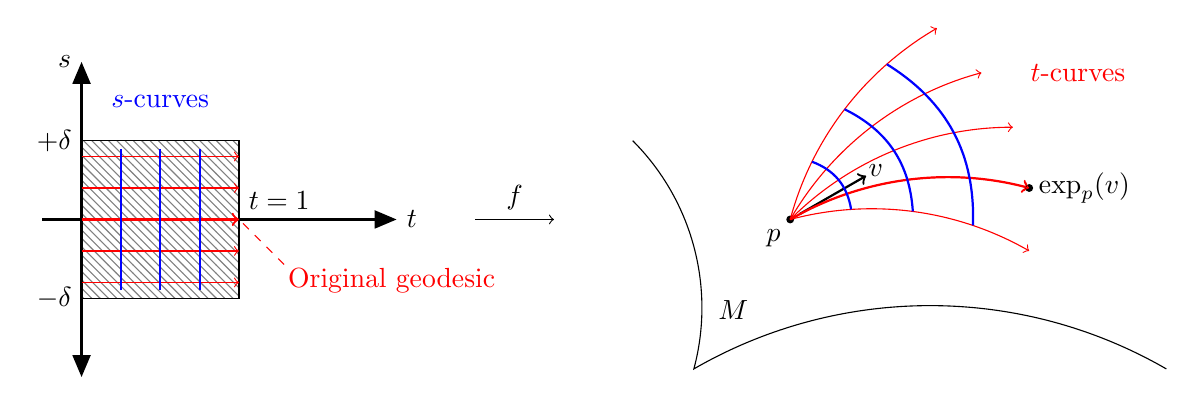
\begin{tikzpicture}
	\draw[pattern=north west lines, pattern color=gray] (0,-1) rectangle (2,1);
	\draw[thick, ->] (-0.5,0) -- (4,0) node[anchor=west]{$t$};
	\draw[thick, <->] (0,-2) -- (0,2) node[anchor=east]{$s$};
	\draw (0,1) node[anchor=east]{$+\delta$} -- (2,1) -- (2,-1) -- (0,-1) node[anchor=east]{$-\delta$};
	\draw[-to, thick, red] (0,0) -- (2,0);
	\draw[-to, red] (0,0.4) -- (2,0.4);
	\draw[-to, red] (0,0.8) -- (2,0.8);
	\draw[-to, red] (0,-0.4) -- (2,-0.4);
	\draw[-to, red] (0,-0.8) -- (2,-0.8);
	\draw[thick, blue] (0.5,-0.9) -- (0.5,0.9);
	\draw[thick, blue] (1,-0.9) -- (1,0.9);
	\draw[thick, blue] (1.5,-0.9) -- (1.5,0.9);
	%
	\draw[-to] (5,0) -- (6,0);
	%
	\draw (7,1) arc (45:-15:3) node (M) {} arc (120:60:6);
	\node (p) at (9,0) {};
	\fill (p) circle [radius=0.05cm];
	\draw (p) + ({1.25*0.87}, {1.25*0.5}) node (v) {};
	\draw[-to, thick] (p) -- (v);
	\draw[-to, red] (p) arc (105:93.75:4) node (s11) {} arc (93.75:82.5:4) node (s21) {} arc (82.5:71.25:4) node (s31) {} arc (71.25:60:4);
	\draw[-to, red, thick] (p) arc (120:75:4) node (exppv) {};
	\draw[-to, red] (p) arc (135:90:4);
	\draw[-to, red] (p) arc (150:105:4) node (tcurve) {};
	\draw[-to, red] (p) arc (165:153.75:4) node (s12) {} arc (153.75:142.5:4) node (s22) {} arc (142.5:131.25:4) node (s32) {} arc (131.25:120:4);
	\fill (exppv) circle [radius=0.05cm];
	\draw[-to, red] (p) arc (120:75:4);
	\draw[blue, thick, bend right=30] (s11.center) to (s12.center);
	\draw[blue, thick, bend right=30] (s21.center) to (s22.center);
	\draw[blue, thick, bend right=30] (s31.center) to (s32.center);
	%
	\draw (5.5,0) node[anchor=south]{$f$};
	\draw (p) node[anchor=north east]{$p$};
	\draw (v) + (0,0) node {$v$};
	\draw (exppv) node[anchor=west]{$\exp_{p}(v)$};
	\draw[red] (tcurve) + (0.5,0) node[anchor=west]{$t$-curves};
	\draw[red] (2.5,-0.5) node[anchor=north west] {Original geodesic};
	\draw[red, dashed] (2.05,-0.05) -- (2.6,-0.6);
	\draw[blue] (1,1.5) node {$s$-curves};
	\draw (2,0) node[anchor=south west]{$t=1$};
	\draw (M) + (0.5,0.75) node{$M$};
\end{tikzpicture}

\par\noindent
If we let $f_{t}=\pd{f}{t}$, the velocity of a $t$-curve, and $f_{s}=\pd{f}{s}$, the velocity of an $s$-curve, then these define vector fields along each $s$ and $t$ curve (respectively).\n

\prop{
	For any family of curves as above, $\frac{D}{dt}f_{s}=\frac{D}{ds}f_{t}$. This follows from the Levi-Civita connection $\nabla$ being torsion-free.\n
}

\par\noindent
$\frac{D}{dt}f_{s}$ is the covariant derivative of the $f_{s}$ vectors along $t$.\n

\end{document}